\IEEEraisesectionheading{\section{Introduction}\label{sec:intro}}

% 场景立意：卫星网络为何天然需要稀疏观测 TE → 三个挑战 → SpaTE 设计 →
% 诚实报告不同观测区间的结果。Fig. 1 恢复为稀疏观测场景图。

\IEEEPARstart{L}{ow-Earth-orbit} (LEO) satellite constellations are rapidly
scaling toward tens of thousands of satellites~\cite{handley2018,
bhattacherjee2019}. Their inter-satellite links (ISLs) carry
spatially concentrated and temporally varying traffic under limited
capacity~\cite{kassing2020}. Traffic engineering (TE), which
coordinates how each demand is split across candidate paths, is therefore
a key control primitive~\cite{jain2013,hong2018}. Classical
optimization can take minutes at constellation scale, whereas learned
allocators reduce online decision time to the sub-second range by moving
most computation offline~\cite{teal,dote,sate}.

Many learned TE systems nevertheless rely on a complete traffic matrix
at every control epoch. This assumption is particularly fragile in an LEO
constellation. Measuring every demand requires satellites to meter,
aggregate, and transmit fine-grained statistics through telemetry channels
that compete with user traffic for ISL and ground-station
bandwidth~\cite{kassing2020,michel2022}. It also consumes onboard
computation, storage, and power, while intermittent ground contacts
introduce unavoidable gaps; the expense of network-wide metering is the very
reason terrestrial operators have long inferred traffic matrices instead of
measuring them~\cite{vardi1996,zhang2003}. As illustrated in
\cref{fig:scenario}, only a subset of satellites may meter traffic at a
given epoch. The controller then receives a sparse traffic matrix but must
still allocate every demand. Efficient TE from sparse observations is thus
a natural operating mode for LEO networks, not merely a degraded version
of complete measurement.

\begin{figure}[t]
    \centering
    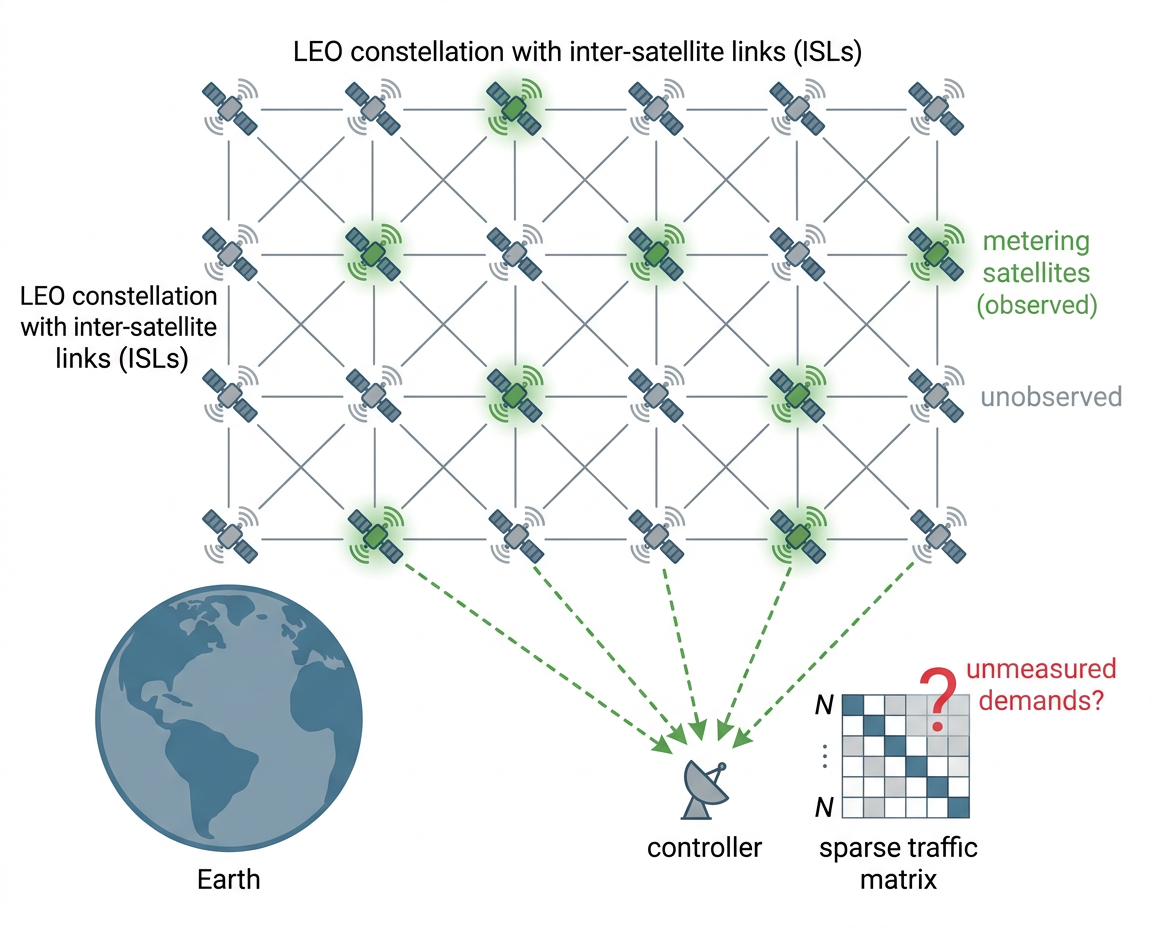
\includegraphics[width=\linewidth]{figures/scenario-draft.png}
    \caption{Sparse traffic observation in an LEO constellation. Only a
    subset of satellites meters traffic, so the controller receives a
    sparse traffic matrix while remaining responsible for all demands.}
    \label{fig:scenario}
\end{figure}

In LEO constellations, sparse observation interacts with geographic traffic
concentration and orbital motion in three ways. First, when metering is
available on only a subset of satellites, an unmeasured source hides a whole
row of demands, not just isolated matrix entries. Since satellites serving
populated footprints can carry substantial traffic~\cite{kassing2020},
zero filling may erase an entire source's contribution to ISL load; explicit
matrix completion instead risks passing reconstruction errors into routing~\cite{zhang2009}.
Second, traffic from nearby footprints shares multi-hop ISL corridors, while
satellite motion changes the association between ground users and ingress
satellites. The allocator must combine current path--link relationships with
recent traffic evolution without allowing imputed values to distort shared
link representations~\cite{t2gnn}. Third, moving footprints change the active
source--destination pairs as the constellation evolves. A model tied to a
fixed demand list would require resizing or retraining, despite the limited
onboard resources and short control windows~\cite{sate}. These coupled
measurement and mobility constraints distinguish sparse-observation TE in
LEO constellations from the static terrestrial setting~\cite{test}.

We present \sysname{} (\underline{Spa}rse-aware \underline{T}raffic
\underline{E}ngineering), a learned allocator designed around these
constraints. It represents each unobserved demand with a learnable mask
embedding rather than a fabricated volume. A mask-gated flow-centric graph
neural network (GNN) lets unobserved demands receive
link-state information without injecting their \emph{placeholders}, the
surrogate values that stand in for unmeasured demands at the model input,
into link embeddings. A temporal Transformer~\cite{vaswani2017} encodes
recent sparse observations, and per-demand cross-attention fuses temporal
and spatial evidence before predicting path split ratios. Shared weights
and demand pruning keep the model independent of the instantaneous demand
set, enabling reuse across constellation snapshots and scales.

After allocation, \sysname{} can optionally refine residual overloads using
link loads estimated from the same sparse observation. The important input
to this lightweight step is a neighbor estimate: an unmeasured demand is
inferred from observed demands sharing its source satellite. This estimate
uses geographic locality to avoid granting the controller an unavailable
ground-truth traffic matrix. It is an implementation aid to the sparse-aware
allocator rather than the organizing principle of the system.

We evaluate \sysname{} on a 1{,}584-satellite Starlink Shell-1
constellation over observation ratios from $2\%$ to $50\%$, measuring the
realized maximum link utilization (MLU) against ground-truth demands. Each
configuration is evaluated through repeated runs with matched random
initializations, separating observation-dependent effects from variation
between runs. \sysname{} holds the
realized MLU in the $1.64$--$1.89$ range, within $1.19$--$1.37\times$ of a
path-restricted LP optimum, while deciding in under $0.4$~s per snapshot and
transferring to a one-third-scale constellation without architectural change.
Against impute-then-optimize pipelines and zero-filled temporal baselines the
outcomes are mixed and no single pairwise comparison reaches significance; we
therefore examine the distributions across repeated runs to identify where
sparse-aware allocation helps and where simple fill-based treatments remain
competitive.

Our contributions are as follows:
\begin{itemize}
    \item We formulate sparse-observation TE for LEO constellations in which
    limited satellite telemetry leaves individual demands or entire source
    rows unmeasured. The formulation separates the controller's partial
    information from the true ISL loads used to evaluate its decisions.
    Predicting path split ratios allows routing decisions for unmeasured
    demands without requiring explicit recovery of their volumes.
    \item We design \sysname{} to combine the spatial structure of ISL routes
    with the recent evolution of geographically concentrated satellite traffic.
    Learnable mask embeddings distinguish missing measurements from zero
    traffic, asymmetric path--link propagation isolates those embeddings from
    measured link evidence, and cross-attention integrates the spatial features
    with sparse observation history. Demand pruning and shared parameters let
    the same architecture accommodate changing active pairs as satellite
    footprints move, without tying its weights to a fixed constellation graph.
    \item We evaluate \sysname{} on a 1{,}584-satellite constellation across
    $2\%$--$50\%$ observability, with a smaller same-family constellation as a
    scale check. Matched comparisons and ablations distinguish the effects of
    sparse-input representation, training, and observation-based refinement.
    The results identify observation-dependent performance and initialization
    sensitivity, bounding the conditions under which the proposed design
    improves MLU instead of assuming a uniform advantage.
\end{itemize}

The remainder of this paper is organized as follows.
\Cref{sec:related} reviews related work. \Cref{sec:formulation} formulates
the sparse-observation TE problem. \Cref{sec:design} presents \sysname{}.
\Cref{sec:eval} evaluates the system, and \cref{sec:conclusion} concludes
the paper.
